\documentclass{beamer}

\usepackage[onehalfspacing]{setspace}
\usepackage[utf8]{inputenc}
\usepackage{gensymb}
\usepackage{url}
\usepackage{mathtools}
\usepackage{booktabs}
\usepackage{graphicx}
\usepackage{tikz}
\usetikzlibrary{shapes.geometric, arrows.meta, positioning}

\usepackage[
backend=biber,
style=numeric,
sorting=ynt,
maxbibnames=12
]{biblatex}
% \addbibresource{Sources.bib}

\usetheme{Madrid}
\usecolortheme{default}

% ------------------------------------------------------------
% Title page information
\title[Neural PK-PD Modeling with ODE]{
Neural PK-PD Modeling with ODE\\
for Early Drug Discovery
}

\subtitle{Master's diploma thesis presentation draft}

\author[]{
Student Name
}

\institute[]{
Faculty / Department Name\\
Warsaw University of Technology
}

\date[June 2026]{June 2026}
% ------------------------------------------------------------

% ------------------------------------------------------------
% Show section TOC at the start of each section
\AtBeginSection[]
{
\begin{frame}
    \frametitle{Table of Contents}
    \tableofcontents[currentsection]
\end{frame}
}
% ------------------------------------------------------------

\begin{document}

\frame{\titlepage}

\begin{frame}
\frametitle{Table of Contents}
\tableofcontents
\end{frame}

% ============================================================
\section{Introduction and Motivation}

\begin{frame}{Problem Context}
\begin{itemize}
    \item Early drug discovery requires simultaneous assessment of \textbf{efficacy}, \textbf{safety}, \textbf{absorption}, and \textbf{elimination}.
    \item Existing studies typically optimize for one or two ADMET endpoints in isolation.
    \item PK-PD modeling and molecular ML are rarely connected within a single reproducible workflow.
    \item Calibration is usually an afterthought, yet uncalibrated probabilities distort downstream risk simulation.
\end{itemize}
\end{frame}

\begin{frame}{Thesis Goal and Research Gap}
\begin{columns}[T]
\begin{column}{0.47\textwidth}
  \small
  \begin{itemize}
    \item Four ADME-Tox endpoints predicted jointly:
    \begin{itemize}\footnotesize
        \item Binding affinity (pIC50)
        \item hERG inhibition (cardiotoxicity)
        \item Caco-2 permeability (absorption)
        \item Hepatic clearance
    \end{itemize}
    \item Single reproducible pipeline: from raw molecules to clinical trial simulation.
    \item Bridge benchmark ML and \textbf{translational decision support}.
  \end{itemize}
\end{column}
\begin{column}{0.50\textwidth}
  \centering
  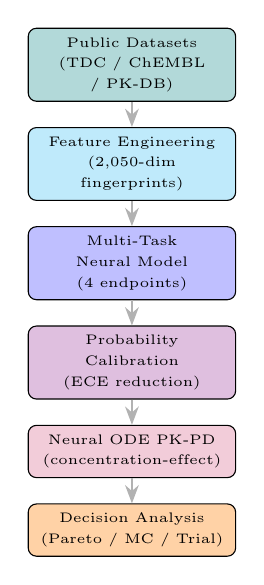
\begin{tikzpicture}[
    s1/.style={draw, rounded corners=3pt, fill=teal!30,
      text width=2.4cm, minimum height=0.52cm, font=\tiny, align=center},
    s2/.style={draw, rounded corners=3pt, fill=cyan!25,
      text width=2.4cm, minimum height=0.52cm, font=\tiny, align=center},
    s3/.style={draw, rounded corners=3pt, fill=blue!25,
      text width=2.4cm, minimum height=0.52cm, font=\tiny, align=center},
    s4/.style={draw, rounded corners=3pt, fill=violet!25,
      text width=2.4cm, minimum height=0.52cm, font=\tiny, align=center},
    s5/.style={draw, rounded corners=3pt, fill=purple!20,
      text width=2.4cm, minimum height=0.52cm, font=\tiny, align=center},
    s6/.style={draw, rounded corners=3pt, fill=orange!35,
      text width=2.4cm, minimum height=0.52cm, font=\tiny, align=center},
    arr/.style={-Stealth, thick, gray!60},
    node distance=0.32cm
  ]
    \node[s1] (d)   {Public Datasets\\ (TDC / ChEMBL / PK-DB)};
    \node[s2, below=of d] (f)   {Feature Engineering\\ (2,050-dim fingerprints)};
    \node[s3, below=of f] (m)   {Multi-Task Neural Model\\ (4 endpoints)};
    \node[s4, below=of m] (c)   {Probability Calibration\\ (ECE reduction)};
    \node[s5, below=of c] (p)   {Neural ODE PK-PD\\ (concentration-effect)};
    \node[s6, below=of p] (dec) {Decision Analysis\\ (Pareto / MC / Trial)};
    \draw[arr] (d)--(f); \draw[arr] (f)--(m);
    \draw[arr] (m)--(c); \draw[arr] (c)--(p);
    \draw[arr] (p)--(dec);
  \end{tikzpicture}
\end{column}
\end{columns}
\end{frame}

% ============================================================
\section{Objectives and Contributions}

\begin{frame}{Four Principal Objectives}
\begin{enumerate}
    \item Build a \textbf{leakage-controlled multi-task dataset} from heterogeneous public sources (TDC, ChEMBL, PK-DB).
    \item Develop predictive models for \textbf{binding, hERG, Caco-2, and clearance} with explicit evaluation of real-data integration and GNN fusion.
    \item Integrate \textbf{calibrated model outputs} with Neural ODE PK-PD simulation for mechanistic analysis.
    \item Evaluate translational behavior via \textbf{Pareto trade-off analysis}, Monte Carlo robustness, and virtual clinical trial simulation.
\end{enumerate}
\end{frame}

\begin{frame}{Key Contributions}
\begin{itemize}
    \item \textbf{Full experimental pipeline}: data curation $\to$ feature engineering $\to$ multi-task training $\to$ calibration $\to$ PK-PD simulation $\to$ decision analysis.
    \item \textbf{Thesis-essential modeling sequence}: TDC fingerprint upgrade $\to$ real ChEMBL binding integration $\to$ hERG refinement $\to$ joint GNN+MLP fusion.
    \item \textbf{Decision-support layer}: Pareto efficacy-safety optimization, Monte Carlo uncertainty quantification, and in-silico clinical trial OC analysis.
    \item \textbf{Exploratory RapidDock prototype}: distance-biased transformer for geometry-aware protein-ligand modeling (feasibility study).
\end{itemize}
\end{frame}

% ============================================================
\section{Data and Modeling Pipeline}

\begin{frame}{Data Sources}
\footnotesize
\begin{tabular}{lrp{4.8cm}}
\hline
\textbf{Source} & \textbf{Rows} & \textbf{Role} \\
\hline
TDC (hERG / Caco-2 / clearance) & 2,768 & Core ADMET benchmark training labels \\
ChEMBL (real-SMILES binding)    & 3,410 & Pharmacodynamic potency (pIC50) \\
PK-DB                           &   796 & Mechanistic ODE calibration context \\
PubChem                         & 5,000 & Illustrative safety screening reference \\
\hline
\end{tabular}
\vspace{0.3cm}
\begin{itemize}\small
  \item \textbf{4,768} harmonized rows, \textbf{4 tasks}, \textbf{2,050 features}.
  \item Split 70\,/\,10\,/\,20; stratified for hERG \& Caco-2.
  \item Quality gate: MD5 deduplication, leakage audit, K-S distribution check.
\end{itemize}
\end{frame}

\begin{frame}{Data Sources -- ChEMBL Binding Affinity}
\centering
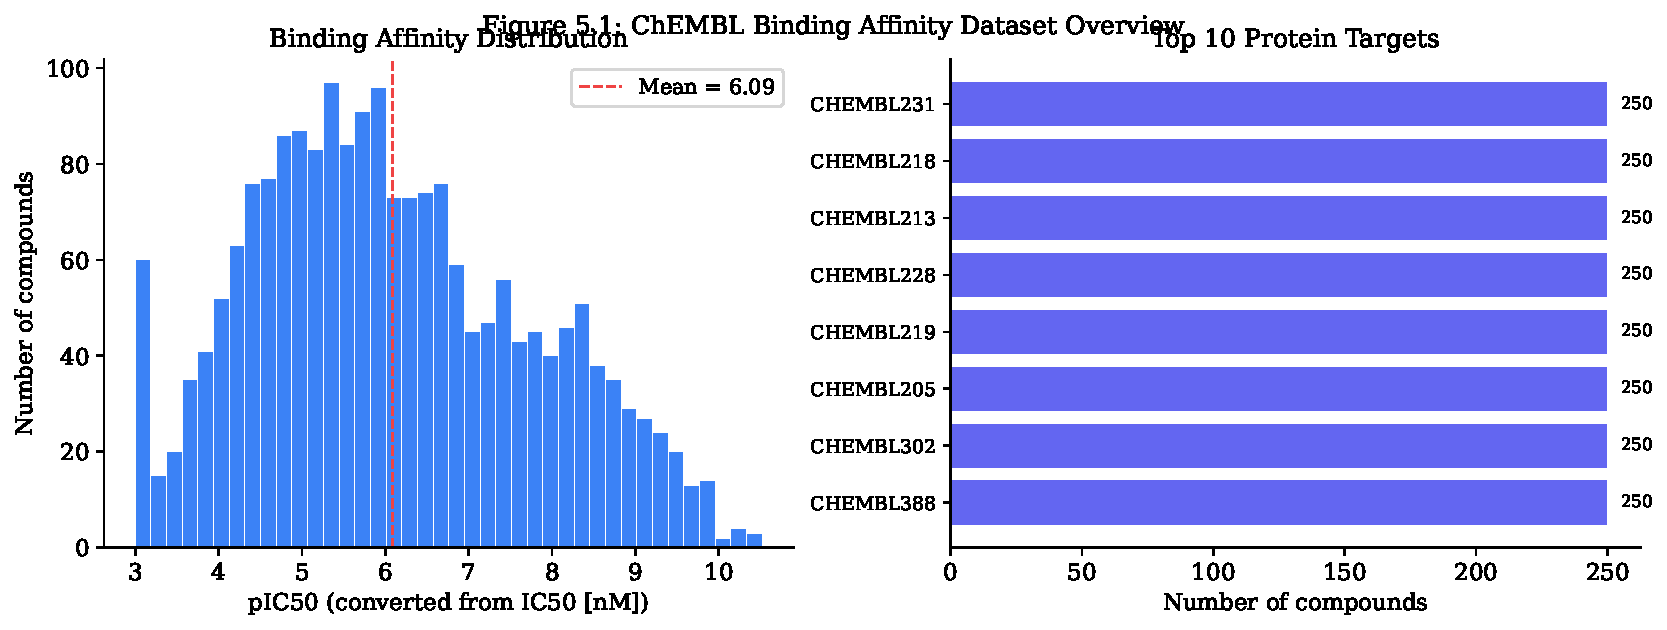
\includegraphics[width=0.97\textwidth, height=0.80\textheight, keepaspectratio]{../Thesis_Latex/2. thesis/figures/fig5_1_chembl_binding.pdf}
\par\vspace{3pt}\footnotesize
pIC50 histogram across 2,000 compounds (left) and top-10 pharmacological target coverage by protein class (right). Mean pIC50\,=\,6.09.
\end{frame}

\begin{frame}{Feature Engineering}
\begin{columns}[T]
\begin{column}{0.44\textwidth}
  \small
  \begin{itemize}
    \item \textbf{Morgan FP}: 2,048 bits, radius 2 (RDKit).
    \item \textbf{Descriptors}: MW, logP.
    \item $\mathbf{x} \in \mathbb{R}^{2050}$.
    \item Task sample counts:
    \begin{itemize}\footnotesize
      \item Binding: 2,000
      \item hERG: 655
      \item Caco-2: 900
      \item Clearance: 1,213
    \end{itemize}
  \end{itemize}
\end{column}
\begin{column}{0.54\textwidth}
  \centering
  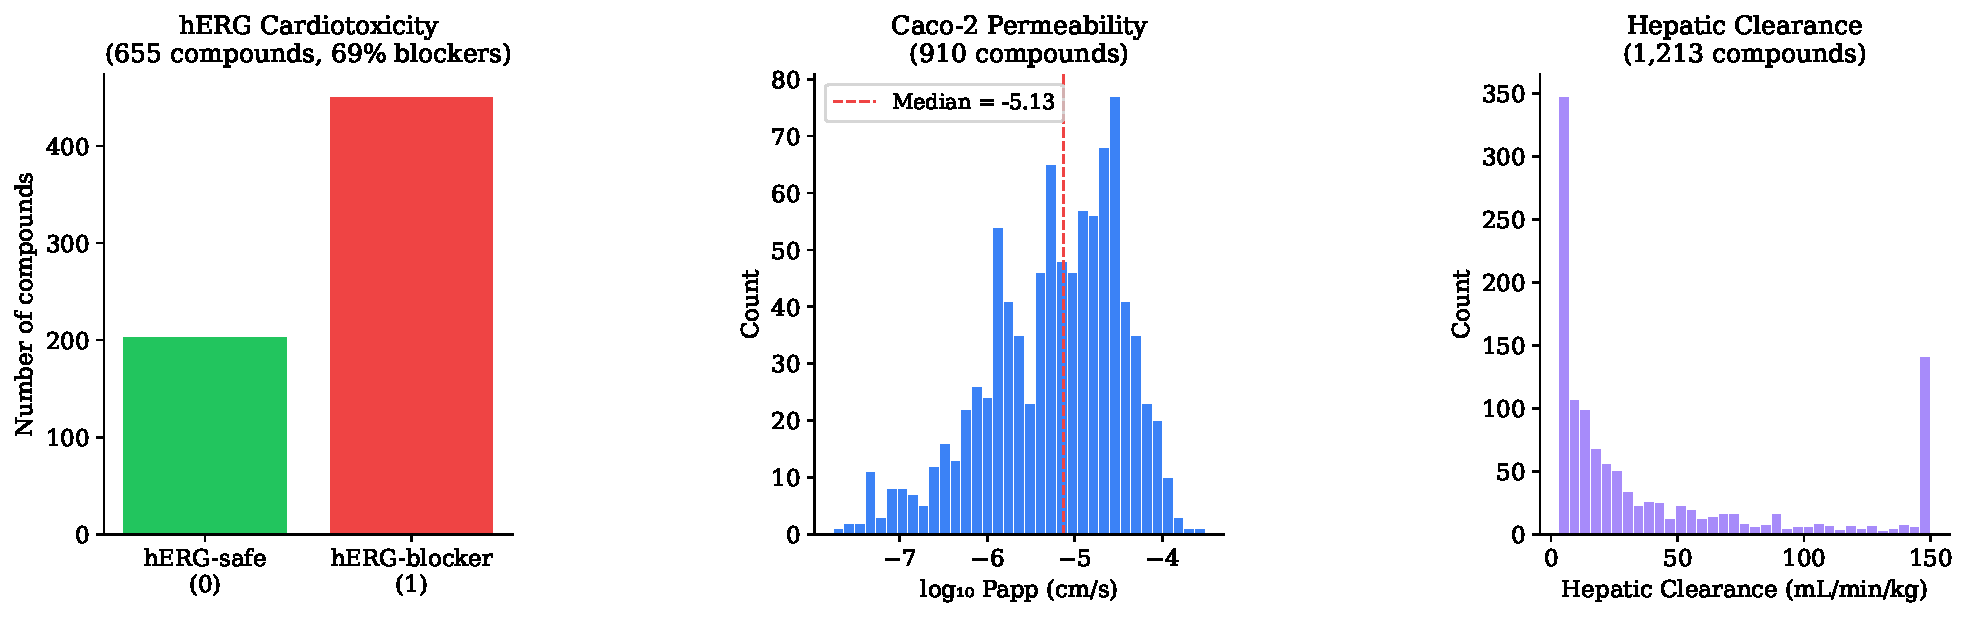
\includegraphics[width=\textwidth]{../Thesis_Latex/2. thesis/figures/fig5_3_tdc_admet.pdf}
  \par\vspace{1pt}\tiny TDC endpoint distributions: hERG class balance (left), Caco-2 permeability (centre), hepatocyte clearance (right).
\end{column}
\end{columns}
\end{frame}

\begin{frame}{Multi-Task Model Architecture}
\begin{columns}[T]
\begin{column}{0.54\textwidth}
  \centering
  \resizebox{0.85\columnwidth}{!}{%
  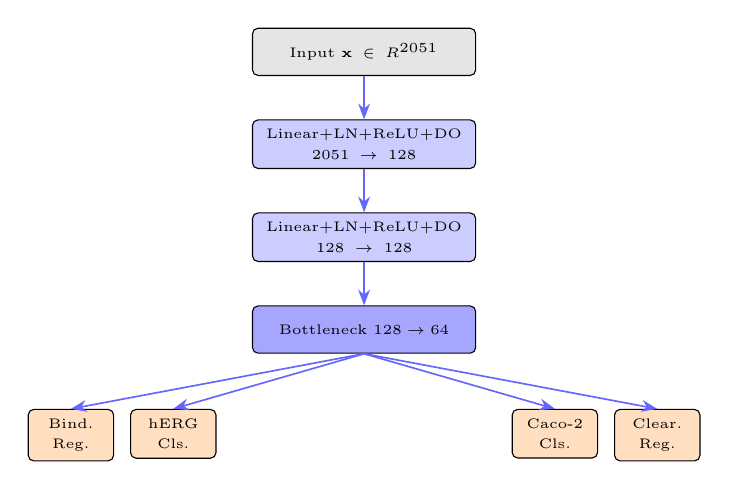
\begin{tikzpicture}[
    enc/.style={draw, rounded corners=2pt, fill=blue!20,
      text width=2.6cm, minimum height=0.60cm, font=\tiny, align=center},
    head/.style={draw, rounded corners=2pt, fill=orange!25,
      text width=0.85cm, minimum height=0.52cm, font=\tiny, align=center},
    arr/.style={-Stealth, semithick, blue!60},
    node distance=0.55cm
  ]
    \node[enc, fill=gray!20] (inp) {Input $\mathbf{x}\in\mathbb{R}^{2051}$};
    \node[enc, below=of inp] (b1) {Linear+LN+ReLU+DO \\ $2051\!\to\!128$};
    \node[enc, below=of b1] (b2) {Linear+LN+ReLU+DO \\ $128\!\to\!128$};
    \node[enc, below=of b2, fill=blue!35] (lat) {Bottleneck $128\!\to\!64$};
    \node[head, below left=0.70cm and 1.75cm of lat] (hd1) {Bind.\\ Reg.};
    \node[head, below left=0.70cm and 0.45cm of lat] (hd2) {hERG\\ Cls.};
    \node[head, below right=0.70cm and 0.45cm of lat] (hd3) {Caco-2\\ Cls.};
    \node[head, below right=0.70cm and 1.75cm of lat] (hd4) {Clear.\\ Reg.};
    \draw[arr] (inp)--(b1); \draw[arr] (b1)--(b2);
    \draw[arr] (b2)--(lat);
    \draw[arr] (lat.south)--(hd1.north);
    \draw[arr] (lat.south)--(hd2.north);
    \draw[arr] (lat.south)--(hd3.north);
    \draw[arr] (lat.south)--(hd4.north);
  \end{tikzpicture}%
  }% end resizebox
\end{column}
\begin{column}{0.44\textwidth}
  \small
  \begin{itemize}
    \item \textbf{Shared encoder}: LayerNorm preferred over BatchNorm for interleaved task batches.
    \item \textbf{Heads from 64-dim bottleneck}:
    \begin{itemize}\footnotesize
      \item Bind: $64\!\to\!64\!\to\!32\!\to\!1$ (deep reg.)
      \item hERG/Caco-2: $64\!\to\!32\!\to\!1$ (logits)
      \item Clearance: $64\!\to\!32\!\to\!1$ (reg.)
    \end{itemize}
    \item \textbf{Loss}: focal ($\gamma{=}2$) + MSE + physics penalty $\mathcal{P}$.
    \item \textbf{Optimizer}: Adam, lr=$10^{-3}$, WD=$10^{-4}$, clip=1.0.
  \end{itemize}
\end{column}
\end{columns}
\end{frame}

\begin{frame}{Calibration and Reliability}
\begin{columns}[T]
\begin{column}{0.44\textwidth}
  \small
  \begin{itemize}
    \item High AUROC $\neq$ reliable probabilities.
    \item hERG \& Caco-2 probabilities feed \textit{directly} into PK-PD as risk variables / $k_a$.
    \item \textbf{Temp.~scaling} (hERG): $\hat{p}=\sigma(z/T)$.
    \item \textbf{Platt scaling} (Caco-2): $\hat{p}=\sigma(az{+}b)$.
  \end{itemize}
  \vspace{0.15cm}
  \footnotesize
  \begin{tabular}{lcc}
  \hline
  \textbf{Task} & \textbf{ECE$_{\text{before}}$} & \textbf{ECE$_{\text{after}}$} \\
  \hline
  hERG (temp.) & 0.1727 & \textbf{0.0058} \\
  Caco-2 (Platt) & 0.3583 & \textbf{0.0448} \\
  \hline
  \end{tabular}
\end{column}
\begin{column}{0.54\textwidth}
  \centering
  
\includegraphics[width=\textwidth]{../Coding/data/outputs/calibration_reliability_s18.png}
  \par\vspace{1pt}\tiny Reliability diagrams: uncalibrated (left), temperature-scaled (centre), Platt-scaled (right). Top row: hERG; bottom row: Caco-2. Diagonal = perfect calibration.
\end{column}
\end{columns}
\end{frame}

% ============================================================
\section{PK-PD and Decision Layer}

\begin{frame}{Endpoint-to-ODE Parameter Mapping}
\footnotesize
\begin{tabular}{lll}
\hline
\textbf{Predicted endpoint} & \textbf{PK/PD role} & \textbf{Parameter} \\
\hline
Clearance (regression) & Elimination rate & $k_e = \text{CL}/V_c$ \\
Caco-2 probability (classif.) & Oral absorption rate & $k_a$ \\
Binding pChEMBL (regression) & PD potency & $EC_{50} = 10^{-\text{pChEMBL}}$ \\
hERG probability (classif.) & Cardiac safety flag & Safety threshold \\
\hline
\end{tabular}
\normalsize
\vspace{0.45cm}
\textbf{Two-compartment PK ODE:}\vspace{-0.25cm}
\begin{equation*}
\frac{dC_c}{dt} = -(k_e + k_{12})C_c + k_{21}C_t + u(t), \quad
\frac{dC_t}{dt} = k_{12}C_c - k_{21}C_t
\end{equation*}
\textbf{Emax PD model:}\vspace{-0.25cm}
\begin{equation*}
E(t) = E_{\max} \cdot \frac{C_c(t)}{EC_{50} + C_c(t)}
\end{equation*}
Solver: \texttt{torchdiffeq.odeint} (Dormand-Prince RK45).
\end{frame}

\begin{frame}{Neural ODE PK-PD Simulation Results}
\centering

\includegraphics[width=0.96\textwidth]{../Coding/data/outputs/pkpd_profiles_s16.png}
\par\vspace{2pt}\footnotesize
Left: 2-compartment PK concentration profiles $C(t)$ for 200 compounds (6 highlighted by pChEMBL and $k_e$). Right: Emax PD effect curves $E(t)$ driven by predicted binding affinity $\to EC_{50}$. Higher pChEMBL $\Rightarrow$ higher sustained effect.
\end{frame}

\begin{frame}{Decision-Layer Analyses}
\begin{columns}[T]
\begin{column}{0.44\textwidth}
  \small
  \begin{itemize}
    \item \textbf{Pareto front}: efficacy vs.\ safety trade-off is genuine---no single dominant regimen.
    \item \textbf{Knee-point}: most balanced point on Pareto frontier.
    \item \textbf{Monte Carlo} ($n{=}1000$): validates regimen robustness; CIs narrow.
    \item \textbf{Virtual trial}: clear dose-response in efficacy; safety burden persists.
  \end{itemize}
\end{column}
\begin{column}{0.54\textwidth}
  \centering
  
\includegraphics[width=\textwidth]{../Coding/data/outputs/s21_risk_benefit.png}
  \par\vspace{1pt}\tiny Scenario risk-benefit map: all regimens exceed safety risk threshold (0.40) while only high-dose regimens surpass efficacy target (12.0). Confirms multi-objective tension.
\end{column}
\end{columns}
\end{frame}

% ============================================================
\section{Results and Discussion}

\begin{frame}{Experimental Progression}
\footnotesize
\begin{tabular}{lp{6.5cm}}
\hline
\textbf{Stage} & \textbf{Key finding} \\
\hline
1. Baseline (256-bit FP) & Near-zero binding $R^2$; hERG AUROC $\approx$ random \\
2. 2048-bit real SMILES & Structural signal enters TDC tasks; clear AUROC lift \\
3. Real ChEMBL binding & Largest binding $R^2$ gain; confirms data-realism bottleneck \\
4. hERG refinement & hidden\_dim $256$ + pos\_weight sweep $\to$ AUROC $>0.80$ \\
5. Calibration & ECE$_{\text{hERG}}$: $0.17\to0.006$; ECE$_{\text{Caco-2}}$: $0.36\to0.045$ \\
6. GNN+MLP fusion & Strongest binding $R^2$; graph+FP representations complementary \\
7--8. PK-PD + Pareto & Genuine efficacy-safety trade-off; knee-point regimen selected \\
9. Monte Carlo & Regimen robustness confirmed; bootstrap CIs narrow \\
10. Virtual trial & Dose-response separation in efficacy; safety burden persists \\
\hline
\end{tabular}
\normalsize
\end{frame}

\begin{frame}{Multi-Task Training Dynamics}
\centering
\includegraphics[width=0.96\textwidth]{../Thesis_Latex/2. thesis/figures/fig8_1_training_history.png}
\par\vspace{2pt}\footnotesize
Left: training and validation loss converge stably across 43 epochs. Right: per-task performance over time---hERG (orange) and Caco-2 (green) AUROC plateau early; binding $R^2$ (blue) grows steadily; clearance $R^2$ (red) improves after initial instability.
\end{frame}

\begin{frame}{GNN+MLP Fusion: Binding Affinity Results}
\centering

\includegraphics[width=0.96\textwidth]{../Coding/data/outputs/joint_gnn_mlp_s19.png}
\par\vspace{2pt}\footnotesize
Left: joint GNN+MLP parity plot ($R^2{=}0.565$, RMSE$=0.722$). Centre: $R^2$ comparison---MLP baseline (S15: 0.452), GNN alone (S17: 0.411), joint fusion (S19: 0.565). Right: joint model learning curve with best val RMSE$=0.781$.
\end{frame}

\begin{frame}{Target Performance Metrics}
\begin{tabular}{lcc}
\hline
\textbf{Task} & \textbf{Metric} & \textbf{Target} \\
\hline
Binding affinity (regression) & $R^2$ & $>0.60$ \\
hERG inhibition (classification) & AUROC & $>0.80$ \\
Caco-2 permeability (classification) & AUROC & $>0.75$ \\
Hepatic clearance (regression) & RMSE & $<1.0$ \\
\hline
\end{tabular}
\vspace{0.3cm}
\begin{itemize}
    \item March 8 baseline reference: hERG AUROC $= 0.4836$, Caco-2 AUROC $= 0.4719$, binding $R^2 = 0.0019$, clearance RMSE $= 0.9766$.
    \item Leakage remediation (MD5 dedup + retrain from scratch on clean splits) was applied before reporting final results.
\end{itemize}
\end{frame}

\begin{frame}{Limitations}
\begin{enumerate}
    \item \textbf{Public data quality}: assay heterogeneity (different protocols, species, cell lines) introduces label noise.
    \item \textbf{ODE parameter assumptions}: $k_{12}$, $k_{21}$ are fixed population averages, not per-compound predictions.
    \item \textbf{GNN scope}: graph encoder trained only for the binding task; other three tasks retain MLP-only heads.
    \item \textbf{No prospective validation}: virtual trial is a model-based planning exercise, not a substitute for empirical data.
    \item \textbf{RapidDock}: exploratory prototype; no calibration, uncertainty quantification, or real PDB protein context.
\end{enumerate}
\end{frame}

\begin{frame}{Conclusions and Future Work}
\begin{itemize}
    \item Real-data integration and GNN+MLP fusion materially improve predictive quality.
    \item Post-hoc calibration is a \textbf{necessary prerequisite} for using classifier probabilities in mechanistic simulation.
    \item The integrated pipeline supports \textbf{multi-objective translational analysis}---Pareto, Monte Carlo, virtual trial---revealing that efficacy gains do not eliminate safety constraints.
\end{itemize}
\vspace{0.2cm}
\textbf{Future work}:
\begin{enumerate}
    \item External and prospective validation.
    \item Per-compound ODE parameter prediction (leverage PK-DB data).
    \item Expanded GNN to all four tasks; extended RapidDock branch with real protein structures.
    \item Interactive deployment as a decision-support tool.
\end{enumerate}
\end{frame}

% ============================================================
\section{Backup}

\begin{frame}{GNN Architecture (Backup)}
\begin{columns}[T]
\begin{column}{0.45\textwidth}
  \small
  \begin{itemize}
    \item \textbf{Atom features}: atomic number (one-hot), degree, formal charge, \#H, aromaticity.
    \item \textbf{Bond features}: type, ring membership.
    \item \textbf{3-layer GCN}:
    \begin{equation*}
      h_v^{(k)} = \text{ReLU}\!\left(W^{(k)} \cdot \text{MeanAGG}_{\mathcal{N}(v)}\right)
    \end{equation*}
    \item \textbf{Fusion}: $z_{\text{fus}} = [z_{\text{GNN}};\, z_{\text{MLP}}]$.
  \end{itemize}
\end{column}
\begin{column}{0.53\textwidth}
  \centering
  
\includegraphics[width=\textwidth]{../Coding/data/outputs/gnn_binding_s17.png}
  \par\vspace{1pt}\tiny GNN binding parity plot ($R^2{=}0.411$) and MPNN training curve vs.\ S15 MLP fingerprint baseline (RMSE $0.822$, dashed).
\end{column}
\end{columns}
\end{frame}

\begin{frame}{RapidDock Prototype (Backup)}
\begin{itemize}
    \item Input: $\sim$80--120 protein-ligand complexes (140 ChEMBL SMILES, RDKit 3D embedding).
    \item \textbf{Distance-biased attention}:
    \begin{equation*}
        \text{Attn}(Q,K,V) = \text{softmax}\!\left(\frac{QK^\top}{\sqrt{d}} - 0.25 \cdot D_{\text{joint}}\right)V
    \end{equation*}
    \item 4 transformer blocks (8 heads, $d_{\text{head}}=16$), learnable type embeddings.
    \item Symmetry-aware distance loss over permutations of same-type atom groups.
    \item Ligand coordinate reconstruction via L-BFGS (200 steps).
    \item \textbf{Status}: feasibility prototype only---no calibration or real PDB structures.
\end{itemize}
\end{frame}

\begin{frame}{Training Hyperparameters (Backup)}
\footnotesize
\begin{tabular}{ll}
\hline
\textbf{Hyperparameter} & \textbf{Value} \\
\hline
Optimizer & Adam \\
Learning rate & $10^{-3}$ (fine-tune: $3\times10^{-4}$) \\
Weight decay & $10^{-4}$ \\
Gradient clip & norm = 1.0 \\
Batch size & 64 \\
Max epochs & 300 \\
Early stopping patience & 40 (extended 60 for hERG sweep) \\
LR scheduler & ReduceLROnPlateau, factor=0.5, patience=10 \\
Focal loss $\gamma$ & 2.0 (hERG, Caco-2) \\
Random seed & 42 \\
\hline
\end{tabular}
\normalsize
\end{frame}

\begin{frame}{Software Stack (Backup)}
\begin{itemize}
    \item Python 3.14
    \item PyTorch 2.10.0 (MPS/CUDA; Neural ODE training)
    \item RDKit 2025.9.5 (fingerprints, SMILES, 3D conformers)
    \item torchdiffeq 0.2.5 (Dormand-Prince RK45 ODE solver)
    \item scikit-learn 1.8.0 (preprocessing, metrics, calibration)
    \item pandas 3.0.0, numpy 2.4.1
    \item Fixed seed (\texttt{SEED=42}) across NumPy, PyTorch, and Python \texttt{random}.
\end{itemize}
\end{frame}

\begin{frame}{Population PK-PD Simulation (Backup)}
\centering

\includegraphics[width=0.96\textwidth]{../Coding/data/outputs/popPKPD_s20.png}
\par\vspace{2pt}\footnotesize
Population simulation ($n{=}500$): A) plasma concentration $C_1(t)$ with 5--95\% uncertainty band; B) PD effect $E(t)$ with IQR band; C) AUC$_E$ distribution (median$=15.97$); D) safety flags---98.2\% of compounds trigger both hERG and Caco-2 safety flags.
\end{frame}

\begin{frame}{Dose Optimization Grid (Backup)}
\centering

\includegraphics[width=0.88\textwidth]{../Coding/data/outputs/s23_dose_optimization.png}
\par\vspace{2pt}\footnotesize
Dose optimization contour maps over dose (mg) vs.\ variability (CV IIV). Top-left: efficacy (AUC$_E$) increases with dose. Top-right: hERG risk ($>$90\% at most doses). Bottom-left: Caco-2 poor-permeability rate. Bottom-right: composite score (green = better). Optimal $\star$ at low dose, low CV.
\end{frame}

\begin{frame}{Sensitivity Analysis -- Tornado Plot (Backup)}
\centering

\includegraphics[width=0.96\textwidth]{../Coding/data/outputs/s22_tornado_plot.png}
\par\vspace{2pt}\footnotesize
Tornado (one-at-a-time $\pm$20\%) sensitivity for three ODE outputs. Left: AUC$_E$ most sensitive to Emax, CL, EC50. Centre: Cmax dominated by dose. Right: AUC$_{C1}$ dominated by CL and dose. Results confirm that predicted CL and binding affinity are the primary levers for PK-PD decisions.
\end{frame}

\begin{frame}
\centering
\Large Thank you
\end{frame}

\end{document}
